\documentclass[12pt,oneside,a4paper]{article}

% a4paper, hocanın a4 seçeneğinin geçerli A4 karşılığıdır.

\usepackage[utf8]{inputenc}
\usepackage[T1]{fontenc}
\usepackage{lmodern}
\usepackage{amssymb,amsmath,graphicx,psfrag}
\usepackage[usenames]{color}
\usepackage[provide=*,turkish]{babel}
\usepackage{fancyhdr,url,array,theorem,subfig,float}
\usepackage{verbatim}
\usepackage{bibentry}

% Diyagramlar ve doğrulama tablosu için ek paketler.
\usepackage{tikz,tabularx,booktabs}
\usepackage[hidelinks]{hyperref}
\captionsetup{font=small,skip=5pt}
\usetikzlibrary{
    arrows.meta,
    positioning,
    shapes.geometric,
    calc,
    babel
}

\newcommand{\parbx}[1]{\parbox{1cm}{\centering #1}}
\newcommand{\parbxx}[1]{\parbox{2cm}{\centering #1}}
\newcommand{\parbxxx}[1]{\parbox{3cm}{\centering #1}}
\newcommand{\parbxxxx}[1]{\parbox{4cm}{\centering #1}}

% ---------------------------------------------------------
% HOCANIN ŞABLONUNDAKİ ÜST VE ALT BİLGİLER
% ---------------------------------------------------------

\pagestyle{fancy}

\fancyfoot[C]{{
    \footnotesize
    Arel Üniversitesi, Müh. Mim Fak.
    Bilgisayar Mühendisliği.
    Türkoba Mahallesi, Erguvan Sokak,
    No:26, K 34537, Tepekent -- Büyükçekmece, İstanbul
}}

\fancyhead[L]{\includegraphics[height=1.1cm]{arel_logo}}
\fancyhead[R]{\thepage}

\renewcommand{\headrulewidth}{0pt}

\graphicspath{{./figures/}}

% ---------------------------------------------------------
% HOCANIN METİN ALANI, OFSETLERİ VE PARAGRAF ARALIĞI
% ---------------------------------------------------------

\setlength{\parindent}{0cm}
\setlength{\parskip}{\baselineskip}

\addtolength{\voffset}{-1cm}
\addtolength{\hoffset}{-1cm}
\addtolength{\textwidth}{1.5cm}
\addtolength{\headwidth}{1cm}
\addtolength{\textheight}{2.8cm}

% Logo için başlık yüksekliği.
% Topmargin telafisi metnin başlangıcını korur.
\setlength{\headheight}{36pt}
\addtolength{\topmargin}{-24pt}

\setlength{\emergencystretch}{2em}

\def\bi{\begin{itemize}}
\def\ei{\end{itemize}}

\AtBeginDocument{%
    \renewcommand{\abstractname}{Özet}%
    \renewcommand{\refname}{Kaynakça}%
    \renewcommand{\figurename}{Şekil}%
    \renewcommand{\tablename}{Tablo}%
}

% ---------------------------------------------------------
% BÜTÜN DİYAGRAMLAR İÇİN ORTAK GÖRSEL DÜZEN
% ---------------------------------------------------------

\definecolor{navy}{HTML}{233F58}
\definecolor{bluebg}{HTML}{EEF3F7}
\definecolor{greenbg}{HTML}{EFF6F0}
\definecolor{amberbg}{HTML}{FFF5E8}
\definecolor{muted}{HTML}{71808E}

\tikzset{
    box/.style={
        draw=navy,
        line width=.65pt,
        fill=bluebg,
        align=center,
        font=\small,
        inner sep=5pt,
        minimum height=9mm
    },
    decision/.style={
        diamond,
        draw=navy,
        line width=.65pt,
        fill=amberbg,
        align=center,
        font=\small,
        aspect=2.2,
        inner sep=2pt
    },
    arrow/.style={
        -{Stealth[length=2mm]},
        draw=navy,
        line width=.75pt
    },
    link/.style={
        {Stealth[length=1.6mm]}-{Stealth[length=1.6mm]},
        draw=muted,
        line width=.55pt
    },
    dependency/.style={
        -{Stealth[open,length=2mm]},
        draw=navy,
        dashed
    },
    usecase/.style={
        ellipse,
        draw=navy,
        line width=.65pt,
        fill=bluebg,
        font=\small,
        align=center,
        text width=4cm,
        inner sep=3pt
    },
    field/.style={
        draw=navy,
        line width=.55pt,
        fill=bluebg,
        align=center,
        font=\small,
        minimum height=11mm,
        inner sep=3pt
    }
}

% ---------------------------------------------------------
% BAŞLIK
% ---------------------------------------------------------

\title{
    C++ ile TCP Tabanlı\\
    Çoklu İstemcili Metin ve Görüntü\\
    Mesajlaşma Uygulaması
}

\author{
    Muhammed Sina Gün\\
    Bilgisayar Mühendisliği\\
    Öğrenci No: 240309910
}

\date{5 Ekim 2026}

\begin{document}
\bibliographystyle{ieeetr}
\maketitle
\thispagestyle{fancy}

% SAYFA 1 - Özet ve mimari
\begin{abstract}
Bu projede, merkezi bir TCP sunucusuna aynı anda en fazla beş
istemcinin bağlanabildiği metin ve görüntü mesajlaşma uygulaması
geliştirilmesi önerilmektedir. Sunucu her bağlantıya benzersiz
kimlik atayacak; kullanıcı aktif istemcileri listeleyip hedef
seçerek yalnız ilgili kullanıcıya metin veya JPG/JPEG/PNG
görüntüsü gönderecektir.

Yazılımın tamamı C++17 ile, Windows 11 üzerinde WSL2 içindeki
Ubuntu 20.04 LTS ortamında geliştirilecektir. TCP akışında ileti
sınırları, tür ve uzunluk alanları içeren 13 baytlık uygulama
başlığıyla belirlenecektir. Kısmi okumalar ve yazmalar döngüyle
tamamlanacak; içerik CRC32 ile denetlenecektir. İstemci başına iş
parçacığı ve hedef başına gönderim kilidi kullanılacaktır.
Başarı; beş aktif bağlantı, doğru hedefe teslim, dosyaların bayt
bayt eşliği ve hataların kontrollü yönetimiyle değerlendirilecektir.
Bu belge tasarım ve deney planını sunmaktadır; ölçülmüş test
sonucu içermemektedir.
\end{abstract}

\begin{figure}[H]
\centering
\begin{tikzpicture}
\node[box,text width=5.4cm,minimum height=13mm] (s) at (0,0)
{\textbf{Merkezi TCP sunucusu}\\5000/TCP - en fazla 5 istemci};
\foreach \n/\x in {1/-5.2,2/-2.6,3/0,4/2.6,5/5.2}
  \node[box,text width=1.85cm,minimum height=12mm] (c\n) at (\x,-2.1)
  {\textbf{İstemci \n}\\Kimlik: \n};
\foreach \n/\x in {1/-2.4,2/-1.2,3/0,4/1.2,5/2.4}
  \draw[link] (c\n.north) -- (\x,-.68);
\draw[arrow,line width=1.1pt] (c1.north) -- (-2.4,-.68);
\draw[arrow,line width=1.1pt] (0,-.68) -- (c3.north);
\node[font=\small,align=center] at (0,-3.1)
{Örnek özel ileti: İstemci 1 $\rightarrow$ Sunucu $\rightarrow$ İstemci 3};
\end{tikzpicture}
\caption{Merkezi mimari ve yalnız seçilen hedefe yapılan aktarım.}
\label{fig:architecture}
\end{figure}

% SAYFA 2 - Giriş, kapsam ve bileşenler
\clearpage
\section{Giriş ve Kapsam}
İstemci-sunucu haberleşmesinde soket yönetimi, ileti çerçeveleme
ve eşzamanlılık birlikte ele alınmalıdır \cite{tanenbaum,kurose}.
Projenin amacı, metin ve görüntüyü tek TCP bağlantısında taşıyan,
özel yönlendirmesi ve hata davranışı açık bir uygulama geliştirmektir.
Şekil~\ref{fig:architecture} merkezi aktarımı göstermektedir.

Kullanıcı listeyi yenileyebilecek, kendisi dışındaki bağlı bir
hedefi seçebilecek ve iki yönde veri gönderebilecektir. Beş etkin
bağlantı varken yeni uygulama bağlantısı reddedilecektir.
Doğrulanan görüntüler \texttt{Alinan\_Dosyalar} dizinine
kaydedilecektir. Hesap sistemi, TLS, veritabanı ve kalıcı sohbet
geçmişi kapsam dışındadır; bağlantı kimliği kullanıcı kimlik
doğrulaması anlamına gelmeyecektir.

\begin{figure}[H]
\centering
\begin{tikzpicture}
\draw[draw=navy,line width=.65pt] (1.9,-2.05) rectangle (9.8,2.05);
\node[font=\small,anchor=north west,fill=white] at (2.1,2.0)
{\textbf{Mesajlaşma uygulaması}};
\draw[draw=navy,line width=.75pt] (0,.08) circle (.18);
\draw[draw=navy,line width=.75pt] (0,-.1) -- (0,-.78);
\draw[draw=navy,line width=.75pt] (-.36,-.34) -- (.36,-.34);
\draw[draw=navy,line width=.75pt] (0,-.78) -- (-.3,-1.12);
\draw[draw=navy,line width=.75pt] (0,-.78) -- (.3,-1.12);
\node[font=\small] at (0,-1.45) {Kullanıcı};
\node[usecase] (u1) at (5.85,1.2) {Aktif istemcileri listele};
\node[usecase] (u2) at (5.85,.3) {Hedef istemciyi seç};
\node[usecase] (u3) at (5.85,-.6) {Özel metin gönder};
\node[usecase] (u4) at (5.85,-1.5) {Özel görüntü gönder};
\foreach \n in {1,2,3,4}
  \draw[draw=navy,line width=.55pt] (.36,-.34) -- (u\n.west);
\end{tikzpicture}
\caption{UML kullanım senaryosu: kullanıcı ve haberleşme işlevleri.}
\label{fig:usecase}
\end{figure}

\begin{figure}[H]
\centering
\begin{tikzpicture}
\node[box,text width=4.2cm] (c) at (0,0)
{\textbf{İstemci}\\\rule{4cm}{.3pt}\\Terminal arayüzü\\Hedef ve dosya seçimi};
\node[box,text width=4.2cm] (s) at (8.2,0)
{\textbf{Sunucu}\\\rule{4cm}{.3pt}\\Aktif istemci listesi\\Bağlantı ve yönlendirme};
\node[box,text width=4.5cm,fill=greenbg] (p) at (4.1,-2.35)
{\textbf{Ortak protokol}\\İleti çerçeveleme\\CRC32 doğrulaması};
\draw[link] (c.east) -- node[above,font=\small]{TCP} (s.west);
\draw[dependency] (c.south) -- (p.north west);
\draw[dependency] (s.south) -- (p.north east);
\end{tikzpicture}
\caption{Bileşenler: istemci, sunucu ve ortak protokol.}
\label{fig:components}
\end{figure}

\section{Çalışma Planı ve Sınırlar}
1. hafta bağlantı ve başlık; 2. hafta metin; 3. hafta görüntü;
4. hafta beş istemci ve özel yönlendirme; 5. hafta deneyler;
6. hafta rapor ve sunum hazırlanacaktır. Dosya adında yol bileşenleri
reddedilecek, UTF-8 bayt uzunluğu denetlenecek ve JPG/PNG imzası
kontrol edilecektir. Başlatılmış çerçeve aktarımı ve gönderim için
30 saniyelik zaman sınırı uygulanacaktır. Sunucu içeriği görebilir;
TLS ve hesap doğrulaması sonraki çalışmalar olarak değerlendirilecektir.

% SAYFA 3 - Yöntem, sıra ve işlem akışı
\clearpage
\section{Yöntem ve İşlem Akışı}
Geliştirme bireysel yürütülecek; uygulama ve deney araçları C++
ile yazılacaktır. Soket yönetiminde UNIX ağ programlama
ilkeleri izlenecektir \cite{stevens}. İlk deneyler
\texttt{127.0.0.1:5000} üzerinde yapılacaktır.

\begin{enumerate}
\setlength{\itemsep}{1pt}\setlength{\parsep}{0pt}
\item \textbf{Bağlantı:} Kabul ve kapasite sayacı birlikte korunacak;
  etkin oturumlara 1--65535 aralığında benzersiz kimlik atanacaktır.
\item \textbf{Aktarım:} Tür ve uzunluklar okunacak; geçerli çerçeve
  tamamen alındıktan sonra CRC32 ve hedef denetlenecektir.
\item \textbf{Hata:} Geçersiz başlık veya yarım kalan çerçevede
  bağlantı kapatılacak; tam okunmuş hatalı iletide hata bildirilecektir.
\item \textbf{Alıcı:} Metin gösterilecek; görüntü geçici dosyaya
  yazılıp doğrulama sonrası tamamlanacaktır. Yarım dosya silinecektir.
\end{enumerate}

\begin{figure}[H]
\centering
\begin{tikzpicture}[font=\small]
\node[box,text width=2.5cm] (a) at (0,0) {\textbf{İstemci 1}};
\node[box,text width=2.5cm] (s) at (5.2,0) {\textbf{Sunucu}};
\node[box,text width=2.5cm] (b) at (10.4,0) {\textbf{İstemci 3}};
\foreach \x in {0,5.2,10.4} \draw[dashed,muted] (\x,-.5) -- (\x,-3.1);
\draw[arrow] (0,-.9) -- node[above]{Liste isteği} (5.2,-.9);
\draw[arrow] (5.2,-1.5) -- node[above]{Aktif kimlikler} (0,-1.5);
\draw[arrow] (0,-2.15) -- node[above]{İleti; hedef: 3} (5.2,-2.15);
\draw[arrow] (5.2,-2.8) -- node[above]{İleti; kaynak: 1} (10.4,-2.8);
\end{tikzpicture}
\caption{Sıra diyagramı: listeleme ve özel iletinin aktarılması.}
\label{fig:sequence}
\end{figure}

\begin{figure}[H]
\centering
\begin{tikzpicture}[font=\small]
\node[box,text width=2.9cm,minimum height=8mm,font=\footnotesize] (a) at (0,0)
{Başlığı tam al\\(13 bayt)};
\node[decision,text width=2.2cm,aspect=3.2,font=\footnotesize] (b) at (0,-1.5)
{Tür/boyut\\uygun mu?};
\node[box,text width=2.9cm,minimum height=8mm,font=\footnotesize] (c) at (0,-3.2)
{Ad ve içeriği\\tam al};
\node[decision,text width=2.2cm,aspect=3.2,font=\footnotesize] (d) at (0,-4.7)
{CRC32/hedef\\uygun mu?};
\node[box,text width=2.9cm,minimum height=8mm,fill=greenbg,font=\footnotesize] (f) at (0,-6.4)
{Hedefe ilet\\(gönderim kilidi)};
\node[box,text width=2.8cm,fill=amberbg,font=\footnotesize] (fatal) at (5.4,-1.5)
{Hata bildir;\\bağlantıyı kapat};
\node[box,text width=2.8cm,fill=amberbg,font=\footnotesize] (recover) at (5.4,-4.7)
{İletiyi reddet;\\hata bildir};
\draw[arrow] (a) -- (b);
\draw[arrow] (b) -- node[left,font=\footnotesize]{Evet} (c);
\draw[arrow] (b.east) -- node[above,font=\footnotesize]{Hayır} (fatal.west);
\draw[arrow] (c) -- (d);
\draw[arrow] (d) -- node[left,font=\footnotesize]{Evet} (f);
\draw[arrow] (d.east) -- node[above,font=\footnotesize]{Hayır} (recover.west);
\draw[arrow] (f.west) -- (-3.3,-6.4) -- (-3.3,0) -- (a.west);
\node[font=\footnotesize,rotate=90,fill=white] at (-3.3,-3.2) {Yeni ileti};
\draw[arrow] (recover.east) -- (7.4,-4.7) -- (7.4,.65) -| (a.north);
\end{tikzpicture}
\caption{Veri iletilerinde hata yolları ve yeni iletiye dönüş.}
\label{fig:activity}
\end{figure}

% SAYFA 4 - Kuramsal temel, protokol ve eşzamanlılık
\clearpage
\section{Kuramsal Temel ve Uygulama Protokolü}
TCP güvenilir, sıralı bir bayt akışıdır; uygulama iletilerinin
sınırlarını korumaz \cite{rfc9293}. Bu nedenle
\texttt{send}/\texttt{recv} dönüşlerindeki bayt sayıları izlenerek
kısmi işlemler tamamlanacaktır \cite{posix}. Cerf ve Kahn'ın
çalışması, ağlar arası iletişimin tarihsel temelini sunmaktadır
\cite{cerf}; uygulama başlığı TCP üzerinde ileti çerçevelemeyi sağlayacaktır.

\begin{figure}[H]
\centering
\begin{tikzpicture}
\node[field,text width=.8cm] (a) {Tür\\1 B};
\node[field,text width=1.5cm,right=0pt of a] (b) {Kimlik\\2 B};
\node[field,text width=1.3cm,right=0pt of b] (c) {Ad uz.\\2 B};
\node[field,text width=1.35cm,right=0pt of c] (d) {Boyut\\4 B};
\node[field,text width=1.3cm,right=0pt of d] (e) {CRC32\\4 B};
\node[field,text width=1.6cm,fill=greenbg,right=0pt of e] (f) {Ad\\$N$ B};
\node[field,text width=1.8cm,fill=greenbg,right=0pt of f] (g) {İçerik\\$D$ B};
\draw[draw=navy,line width=.55pt] (a.north west) -- ++(0,.22) -| (e.north east);
\node[font=\footnotesize,anchor=south]
at ($(a.north west)!.5!(e.north east)+(0,.22)$) {Sabit başlık: 13 bayt};
\end{tikzpicture}
\caption{13 baytlık başlık; toplam çerçeve uzunluğu $13+N+D$ bayttır.}
\label{fig:frame}
\end{figure}

\begingroup\small
\renewcommand{\arraystretch}{1.03}
\begin{tabularx}{\linewidth}{@{}l>{\raggedright\arraybackslash}p{3.0cm}>{\raggedright\arraybackslash}X@{}}
\toprule
\textbf{Tür} & \textbf{İşlev} & \textbf{Alan kuralları}\\
\midrule
\texttt{0x01} & Liste isteği & Kimlik, $N$ ve $D$ sıfırdır.\\
\texttt{0x02} & Metin & $N=0$; $1\leq D\leq64$ KiB; UTF-8.\\
\texttt{0x03} & Görüntü & $1\leq N\leq255$; $1\leq D\leq10$ MiB.\\
\texttt{0x10} & Kimlik bildirimi & $N=0$; $D=2$; atanmış kimlik içeriktedir.\\
\texttt{0x11} & Liste yanıtı & $N=0$; içerik: 1 bayt sayı ve 2 baytlık kimlikler.\\
\texttt{0x12} & Hata bildirimi & $N=0$; en çok 4 KiB UTF-8 hata açıklaması.\\
\bottomrule
\end{tabularx}
\endgroup

Türler yönlerine göre denetlenecek; çok baytlı sayılar ağ bayt
sırasında ayrı ayrı serileştirilecektir.
Veri iletisinde kimlik alanı, istemciden sunucuya \emph{hedefi},
sunucudan alıcıya \emph{kaynağı} gösterecektir. Kaynak kimliği
sunucu bağlantı kaydından alacaktır; kontrol iletilerinde alan
sıfır olacaktır. CRC32, dosya adı ve içerik baytları üzerinde
PNG'deki CRC32 yöntemiyle hesaplanacaktır \cite{png}; boş içerikte
sıfırdır. Bu denetim kesin bütünlük, şifreleme veya kimlik
doğrulama garantisi değildir.

Her bağlantı ayrı iş parçacığında yönetilecektir. İstemci listesi
kilitle korunacak; Şekil~\ref{fig:concurrency}'deki hedef kilidi
başlık, ad ve içeriğin tamamı yazılana kadar tutulacaktır.
Liste kilidi ağ işlemleri boyunca tutulmayacak; kapanan
bağlantının kaydı ve kaynakları güvenli biçimde kaldırılacaktır.

\begin{figure}[H]
\centering
\begin{tikzpicture}
\node[box,text width=2.5cm,font=\footnotesize] (a) at (0,.65)
{Bağlantı A\\İş parçacığı};
\node[box,text width=2.5cm,font=\footnotesize] (b) at (0,-.65)
{Bağlantı B\\İş parçacığı};
\node[box,text width=2.7cm,fill=amberbg,font=\footnotesize] (m) at (5.1,0)
{Hedefin\\gönderim kilidi};
\node[box,text width=2.5cm,fill=greenbg,font=\footnotesize] (s) at (10.2,0)
{Hedef istemci\\TCP soketi};
\draw[arrow] (a.east) -- (m.north west);
\draw[arrow] (b.east) -- (m.south west);
\draw[arrow] (m) -- node[above,font=\footnotesize]{Tam çerçeve} (s);
\end{tikzpicture}
\caption{Aynı hedefe yazılan çerçevelerin birbirine karışmasını önleyen kilit.}
\label{fig:concurrency}
\end{figure}

% SAYFA 5 - Planlanan testler, çalışma planı ve kaynakça
\clearpage
\section{Beklenen Sonuçlar ve Doğrulama Planı}
Deneyler tek bilgisayarda, ayrı sunucu ve istemci süreçleriyle
yürütülecektir. Her senaryo 10 kez tekrarlanacak; koşul, sonuç,
bayt sayısı ve aktarım süresi kaydedilecektir. Tablo~\ref{tab:validation}
planlanan kabul ölçütlerini göstermektedir.

\begin{table}[H]
\centering
\caption{Planlanan deneyler ve kabul ölçütleri; ölçülmüş sonuç değildir.}
\label{tab:validation}
\footnotesize\renewcommand{\arraystretch}{1.06}
\begin{tabularx}{\linewidth}{@{}>{\raggedright\arraybackslash}p{3.15cm}>{\raggedright\arraybackslash}X@{}}
\toprule
\textbf{Deney} & \textbf{Kabul ölçütü}\\
\midrule
Kapasite ve liste & 5 etkin istemci; 6. uygulama bağlantısı reddedilir.
Ayrılma sonrası liste güncellenir, boş yere yeni istemci kabul edilir.\\
Özel metin ve hedef & Türkçe metin yalnız hedefe ulaşır; kendi kimliğine
ve bağlı olmayan hedefe gönderim reddedilir.\\
Görüntü ve eşlik & 1, 5 ve 10 MiB JPG/PNG dosyaları alıcıda
kaynakla bayt bayt aynıdır; kısmi dosya tamamlanmış sayılmaz.\\
Parçalı ve eşzamanlı & Başlık/içerik küçük parçalarda gönderilir;
2 göndericinin aynı hedefe iletileri eksiksiz ayrıştırılır.\\
CRC ve sınır değerleri & Yanlış CRC reddedilir; 64 KiB metin/10 MiB
görüntü kabul edilir; sınırın 1 bayt üstü ve geçersiz tür reddedilir.\\
Kesinti ve dosya adı & Aktarımda bağlantı kopması/zaman aşımı uygulamayı
çökertmez; dizin geçişi ve mevcut dosyanın üzerine yazma engellenir.\\
\bottomrule
\end{tabularx}
\end{table}

Başarı oranı, kabul ölçütünü sağlayan koşu sayısının toplam koşuya
oranı olarak raporlanacaktır. Görüntü aktarımında ilk gönderimden
alıcıdaki doğrulama ve kaydın tamamlanmasına kadar süre ölçülecek;
ortalama ve en yüksek süre ile $D/\text{süre}$ veri hızı verilecektir. Geri döngü
ölçümleri gerçek ağ performansına genellenmeyecektir.

\begingroup\footnotesize
\begin{thebibliography}{9}
\setlength{\itemsep}{2pt}\setlength{\parsep}{0pt}
\bibitem{tanenbaum}
A. S. Tanenbaum ve D. J. Wetherall, \emph{Computer Networks},
5. baskı. Pearson Prentice Hall, 2011.
\bibitem{kurose}
J. F. Kurose ve K. W. Ross, \emph{Computer Networking: A Top-Down
Approach}, 8. baskı. Pearson, 2021.
\bibitem{stevens}
W. R. Stevens, B. Fenner ve A. M. Rudoff, \emph{UNIX Network
Programming, Volume 1: The Sockets Networking API}, 3. baskı.
Addison-Wesley, 2004.
\bibitem{rfc9293}
W. Eddy (ed.), ``Transmission Control Protocol (TCP),'' RFC 9293,
Ağustos 2022. \url{https://www.rfc-editor.org/rfc/rfc9293}
\bibitem{posix}
IEEE ve The Open Group, \emph{The Open Group Base Specifications,
Issue 8}, ``recv'' ve ``send,'' 2024.
\url{https://pubs.opengroup.org/onlinepubs/9799919799/functions/recv.html}
\bibitem{cerf}
V. G. Cerf ve R. E. Kahn, ``A Protocol for Packet Network
Intercommunication,'' \emph{IEEE Transactions on Communications},
cilt 22, sayı 5, ss. 637--648, 1974. doi: 10.1109/TCOM.1974.1092259.
\bibitem{png}
W3C, \emph{Portable Network Graphics (PNG) Specification},
3. baskı, bölüm 5.5, 2025. \url{https://www.w3.org/TR/png-3/}
\end{thebibliography}
\endgroup
\end{document}
